\documentclass{standalone}
\usepackage{tikz}
\usetikzlibrary{patterns, positioning}


\begin{document}
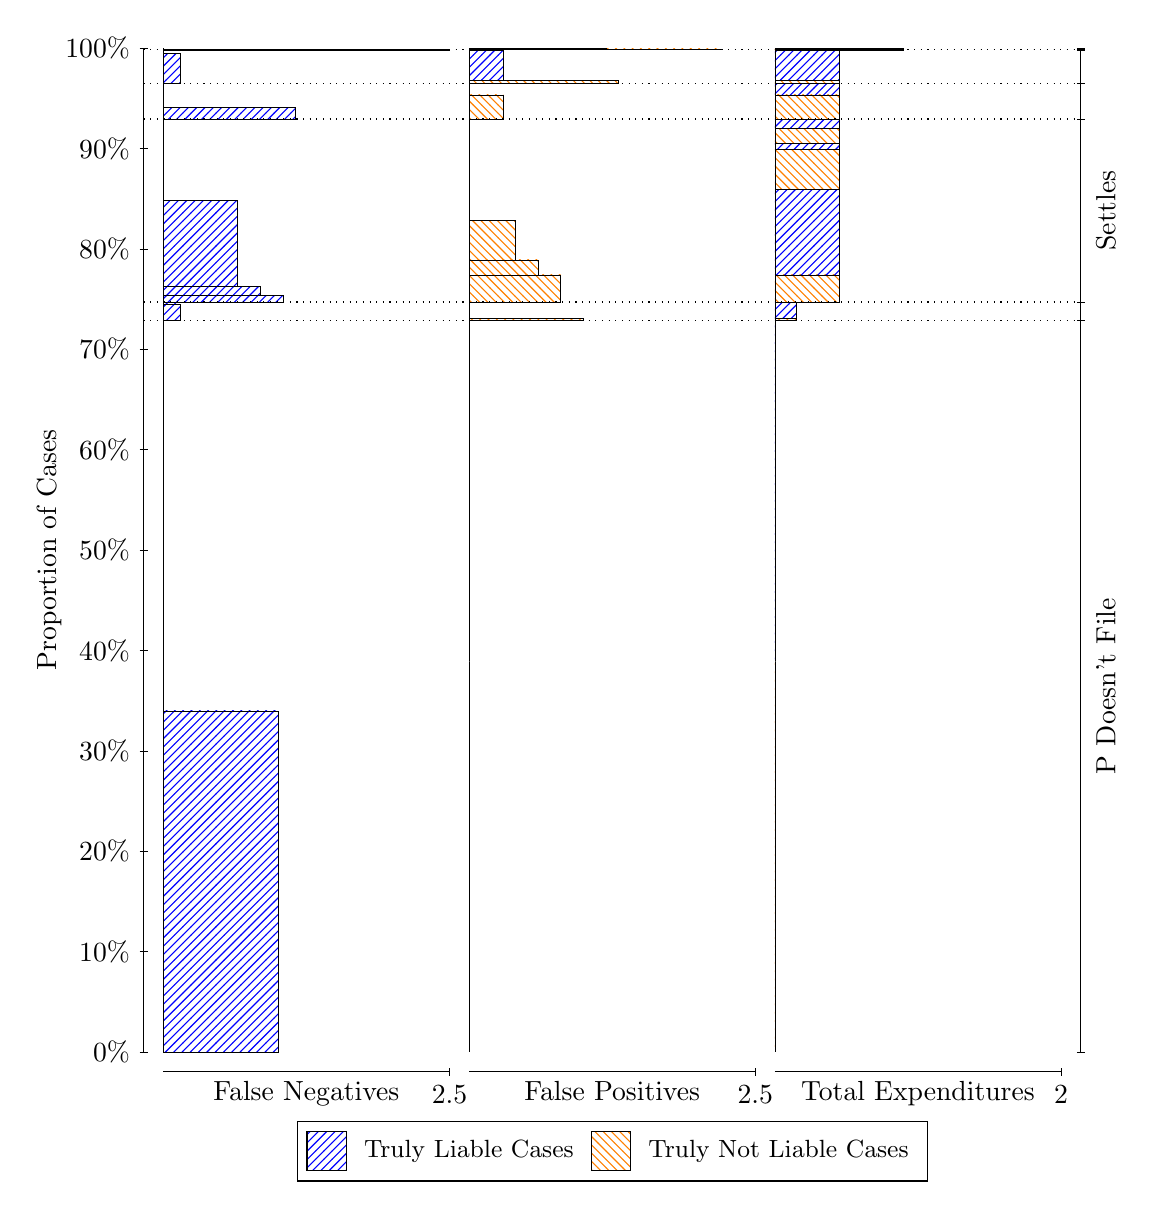
\begin{tikzpicture}
\draw[black, very thin] (1.5,1.75) -- (1.5,14.5);
\node[rotate=90, text=black, anchor=center] at (0.3, 8.125) {Proportion of Cases};
\draw[black, very thin] (1.45,1.75) -- (1.55,1.75);
\node[text=black, anchor=east] at (1.45, 1.75) {0\%};
\draw[black, very thin] (1.45,3.025) -- (1.55,3.025);
\node[text=black, anchor=east] at (1.45, 3.025) {10\%};
\draw[black, very thin] (1.45,4.3) -- (1.55,4.3);
\node[text=black, anchor=east] at (1.45, 4.3) {20\%};
\draw[black, very thin] (1.45,5.575) -- (1.55,5.575);
\node[text=black, anchor=east] at (1.45, 5.575) {30\%};
\draw[black, very thin] (1.45,6.85) -- (1.55,6.85);
\node[text=black, anchor=east] at (1.45, 6.85) {40\%};
\draw[black, very thin] (1.45,8.125) -- (1.55,8.125);
\node[text=black, anchor=east] at (1.45, 8.125) {50\%};
\draw[black, very thin] (1.45,9.4) -- (1.55,9.4);
\node[text=black, anchor=east] at (1.45, 9.4) {60\%};
\draw[black, very thin] (1.45,10.675) -- (1.55,10.675);
\node[text=black, anchor=east] at (1.45, 10.675) {70\%};
\draw[black, very thin] (1.45,11.95) -- (1.55,11.95);
\node[text=black, anchor=east] at (1.45, 11.95) {80\%};
\draw[black, very thin] (1.45,13.225) -- (1.55,13.225);
\node[text=black, anchor=east] at (1.45, 13.225) {90\%};
\draw[black, very thin] (1.45,14.5) -- (1.55,14.5);
\node[text=black, anchor=east] at (1.45, 14.5) {100\%};

\draw[black, very thin] (13.4,1.75) -- (13.4,14.5);
\draw[black, very thin] (13.35,1.75) -- (13.45,1.75);
\node[anchor=west] at (13.35, 1.75) {};
\draw[black, very thin] (13.35,11.041) -- (13.45,11.041);
\node[anchor=west] at (13.35, 11.041) {};
\draw[black, very thin] (13.35,11.274) -- (13.45,11.274);
\node[anchor=west] at (13.35, 11.274) {};
\draw[black, very thin] (13.35,13.598) -- (13.45,13.598);
\node[anchor=west] at (13.35, 13.598) {};
\draw[black, very thin] (13.35,14.05) -- (13.45,14.05);
\node[anchor=west] at (13.35, 14.05) {};
\draw[black, very thin] (13.35,14.476) -- (13.45,14.476);
\node[anchor=west] at (13.35, 14.476) {};
\draw[black, very thin] (13.35,14.484) -- (13.45,14.484);
\node[anchor=west] at (13.35, 14.484) {};
\draw[black, very thin] (13.35,14.5) -- (13.45,14.5);
\node[anchor=west] at (13.35, 14.5) {};

\draw[black, very thin, pattern color=blue, pattern=north east lines] (1.75,1.75) rectangle (3.2033,6.0831);
\draw[black, very thin, pattern color=orange, pattern=north west lines] (1.75,6.0831) rectangle (1.75,11.041);
\draw[black, very thin, pattern color=blue, pattern=north east lines] (1.75,11.041) rectangle (1.968,11.25);
\draw[black, very thin, pattern color=orange, pattern=north west lines] (1.75,11.25) rectangle (1.75,11.274);
\draw[black, very thin, pattern color=blue, pattern=north east lines] (1.75,11.274) rectangle (3.276,11.354);
\draw[black, very thin, pattern color=blue, pattern=north east lines] (1.75,11.354) rectangle (2.9853,11.476);
\draw[black, very thin, pattern color=blue, pattern=north east lines] (1.75,11.476) rectangle (2.6947,12.561);
\draw[black, very thin, pattern color=orange, pattern=north west lines] (1.75,12.561) rectangle (1.75,13.598);
\draw[black, very thin, pattern color=blue, pattern=north east lines] (1.75,13.598) rectangle (3.4213,13.744);
\draw[black, very thin, pattern color=orange, pattern=north west lines] (1.75,13.744) rectangle (1.75,14.05);
\draw[black, very thin, pattern color=blue, pattern=north east lines] (1.75,14.05) rectangle (1.968,14.434);
\draw[black, very thin, pattern color=orange, pattern=north west lines] (1.75,14.434) rectangle (1.75,14.476);
\draw[black, very thin, pattern color=blue, pattern=north east lines] (1.75,14.476) rectangle (5.3833,14.48);
\draw[black, very thin, pattern color=orange, pattern=north west lines] (1.75,14.48) rectangle (1.75,14.484);
\draw[black, very thin, pattern color=orange, pattern=north west lines] (1.75,14.484) rectangle (1.75,14.488);
\draw[black, very thin, pattern color=blue, pattern=north east lines] (1.75,14.488) rectangle (1.75,14.5);
\draw[black, very thin, pattern color=orange, pattern=north west lines] (5.6333,1.75) rectangle (5.6333,6.7077);
\draw[black, very thin, pattern color=blue, pattern=north east lines] (5.6333,6.7077) rectangle (5.6333,11.041);
\draw[black, very thin, pattern color=orange, pattern=north west lines] (5.6333,11.041) rectangle (7.0867,11.065);
\draw[black, very thin, pattern color=blue, pattern=north east lines] (5.6333,11.065) rectangle (5.6333,11.274);
\draw[black, very thin, pattern color=orange, pattern=north west lines] (5.6333,11.274) rectangle (6.796,11.62);
\draw[black, very thin, pattern color=orange, pattern=north west lines] (5.6333,11.62) rectangle (6.5053,11.809);
\draw[black, very thin, pattern color=orange, pattern=north west lines] (5.6333,11.809) rectangle (6.2147,12.312);
\draw[black, very thin, pattern color=blue, pattern=north east lines] (5.6333,12.312) rectangle (5.6333,13.598);
\draw[black, very thin, pattern color=orange, pattern=north west lines] (5.6333,13.598) rectangle (6.0693,13.904);
\draw[black, very thin, pattern color=blue, pattern=north east lines] (5.6333,13.904) rectangle (5.6333,14.05);
\draw[black, very thin, pattern color=orange, pattern=north west lines] (5.6333,14.05) rectangle (7.5227,14.092);
\draw[black, very thin, pattern color=blue, pattern=north east lines] (5.6333,14.092) rectangle (6.0693,14.476);
\draw[black, very thin, pattern color=orange, pattern=north west lines] (5.6333,14.476) rectangle (5.6333,14.48);
\draw[black, very thin, pattern color=blue, pattern=north east lines] (5.6333,14.48) rectangle (5.6333,14.484);
\draw[black, very thin, pattern color=orange, pattern=north west lines] (5.6333,14.484) rectangle (8.8307,14.488);
\draw[black, very thin, pattern color=blue, pattern=north east lines] (5.6333,14.488) rectangle (7.3773,14.5);
\draw[black, very thin, pattern color=orange, pattern=north west lines] (9.5167,1.75) rectangle (9.5167,6.7077);
\draw[black, very thin, pattern color=blue, pattern=north east lines] (9.5167,6.7077) rectangle (9.5167,11.041);
\draw[black, very thin, pattern color=orange, pattern=north west lines] (9.5167,11.041) rectangle (9.7892,11.065);
\draw[black, very thin, pattern color=blue, pattern=north east lines] (9.5167,11.065) rectangle (9.7892,11.274);
\draw[black, very thin, pattern color=orange, pattern=north west lines] (9.5167,11.274) rectangle (10.334,11.62);
\draw[black, very thin, pattern color=blue, pattern=north east lines] (9.5167,11.62) rectangle (10.334,12.705);
\draw[black, very thin, pattern color=orange, pattern=north west lines] (9.5167,12.705) rectangle (10.334,13.208);
\draw[black, very thin, pattern color=blue, pattern=north east lines] (9.5167,13.208) rectangle (10.334,13.287);
\draw[black, very thin, pattern color=orange, pattern=north west lines] (9.5167,13.287) rectangle (10.334,13.476);
\draw[black, very thin, pattern color=blue, pattern=north east lines] (9.5167,13.476) rectangle (10.334,13.598);
\draw[black, very thin, pattern color=orange, pattern=north west lines] (9.5167,13.598) rectangle (10.334,13.904);
\draw[black, very thin, pattern color=blue, pattern=north east lines] (9.5167,13.904) rectangle (10.334,14.05);
\draw[black, very thin, pattern color=orange, pattern=north west lines] (9.5167,14.05) rectangle (10.334,14.092);
\draw[black, very thin, pattern color=blue, pattern=north east lines] (9.5167,14.092) rectangle (10.334,14.476);
\draw[black, very thin, pattern color=orange, pattern=north west lines] (9.5167,14.476) rectangle (11.152,14.48);
\draw[black, very thin, pattern color=blue, pattern=north east lines] (9.5167,14.48) rectangle (11.152,14.484);
\draw[black, very thin, pattern color=orange, pattern=north west lines] (9.5167,14.484) rectangle (11.152,14.488);
\draw[black, very thin, pattern color=blue, pattern=north east lines] (9.5167,14.488) rectangle (11.152,14.5);
\draw[black, dotted] (1.5,11.041) -- (13.4,11.041);
\draw[black, dotted] (1.5,11.274) -- (13.4,11.274);
\draw[black, dotted] (1.5,13.598) -- (13.4,13.598);
\draw[black, dotted] (1.5,14.05) -- (13.4,14.05);
\draw[black, dotted] (1.5,14.476) -- (13.4,14.476);
\draw[black, dotted] (1.5,14.484) -- (13.4,14.484);
\draw[black, very thin] (1.75,1.5) -- (5.3833,1.5);
\node[text=black, anchor=north] at (3.5667, 1.5) {False Negatives};
\draw[black, very thin] (5.3833,1.45) -- (5.3833,1.55);
\node[text=black, anchor=north] at (5.3833, 1.45) {2.5};

\draw[black, very thin] (5.6333,1.5) -- (9.2667,1.5);
\node[text=black, anchor=north] at (7.45, 1.5) {False Positives};
\draw[black, very thin] (9.2667,1.45) -- (9.2667,1.55);
\node[text=black, anchor=north] at (9.2667, 1.45) {2.5};

\draw[black, very thin] (9.5167,1.5) -- (13.15,1.5);
\node[text=black, anchor=north] at (11.333, 1.5) {Total Expenditures};
\draw[black, very thin] (13.15,1.45) -- (13.15,1.55);
\node[text=black, anchor=north] at (13.15, 1.45) {2};

\node[text=black, centered, rotate=90] at (13.72, 6.3954) {P Doesn't File};

\node[text=black, centered, rotate=90] at (13.72, 12.436) {Settles};





\draw (7.449999999999999,1.5) node[draw=none] (baseCoordinate) {};
\begin{scope}[align=center]
        \matrix[scale=0.5, draw=black, below=0.5cm of baseCoordinate, nodes={draw}, column sep=0.1cm]{
            \node[rectangle, draw, minimum width=0.5cm, minimum height=0.5cm, pattern color=blue, pattern=north east lines] {}; &
            \node[draw=none, font=\small, text=black] (B) {Truly Liable Cases}; &
            \node[rectangle, draw, minimum width=0.5cm, minimum height=0.5cm, pattern color=orange, pattern=north west lines] {}; &
            \node[draw=none, font=\small, text=black] (B) {Truly Not Liable Cases}; \\
            };
\end{scope}

\end{tikzpicture}
\end{document}